% 模板名称:vim-latex-elegantbook
% 模板作者: 冯振华
% 电子邮箱:fengzhenhua@outlook.com
% 文件名称: 群论.tex
% 创建时间: 2022年09月13日 星期二 22时38分50秒 
% 创建主机:feng@archlinux
%%%% 可用选项%%%%
% 语言环境:lang=cn,en
% 主题颜色:color=green,cyan,blue,gray,black
% 页面设置:device=pad,normal (A4纸)
% 标题风格:titlestyle=hang,display
% 章节编号:scheme=chinese 默认为阿拉伯数字
% 参考文献:bibend=biber,bibtex
% 目录选项:toc=onecol,twocol
% 旁注选项:margingpar=margintrue
% 数学字体:math=cm,newtx,mtpro2
% 定理模式:mode=simple,fancy
%%% 内置命令 %%%%
% \lstinline{foo}:用于强调提示
%%%% 内置环境 %%%%
% 定理类环境:definition, theorem,lemma,corollary, proposition
% 示例类环境:example,problem,exercise
% 提示类环境:note
% 结论类环境:conclusion,assumption,property,remark,solution
%%%% 默认图片 %%%%
% \cover{~/图片/ElegantPicture/00.jpg} 
%       以数字编号00到09,格式均为jpg, 源自https://pixabay.com/photos/
% \logo{~/图片/ElegantPicture/logo.png} 
%       目前有:logo.png,bnu.jpg,dzu.eps
%
\documentclass[math=mtpro2,lang=cn,color=green,device=pad]{elegantbook}
\usepackage{xeCJKfntef}
\usepackage{float}
%\usepackage[user=teacher]{cexam}
\begin{document}
\title{群论}
\subtitle{田强\& 教8楼 106}
\author{冯振华}
\date{2022年09月13日}
\version{V1.0}
\cover{./ElegantPicture/04.jpg}
\logo{./ElegantPicture/bnu.jpg}
\institute{北京师范大学}
\extrainfo{学为人师,行为世范}
\maketitle
\frontmatter
\tableofcontents
\mainmatter

\chapter{群的基本概念}

\section{简介}

教材和主要内容:《群论及其在固体物理中的应用》 (徐婉棠、喀兴林) 高等教育出版社

群论:关于对称性的数学理论

对称性的描述:对称操作,其包括转动、镜面反映、中心反演

\begin{enumerate}
   \item 转动: $C_n$ 表示绕一个轴转动$\frac{2\pi}{n}$,基中以$E$表示不动
   \item 镜面:关于某个轴镜面对称,以$\sigma$表示,比如$\sigma_y$ 表示以为$y$为对称轴镜面对称,即$\sigma_y : x\rightarrow -x$
   \item 中心反演:$\vec{r}\rightarrow -\vec{r}$
\end{enumerate}

\section{群举例}

\subsection{长方形群}

\begin{figure}[H]
   \centering
   \begin{tikzpicture}
      \draw (0,0) rectangle (3,2); 
      \draw[dashed] (-0.5,1)--(3.5,1) ;
      \draw (3.5,1) node [anchor=west] {$\sigma_x$};
      \draw[dashed] (1.5,-0.5)--(1.5,2.5) ;
      \draw (1.5,2.5) node [anchor=south] {$\sigma_y$};
      \draw (1.5,1) node [anchor=south east] {$O$};
   \end{tikzpicture}
   \caption{长方式形群}
   \label{fig:group1}
\end{figure}

长方形群表示为:$\left\{ E , C_2, \sigma_x, \sigma_y  \right\}$ , 其中$O$点为其反演中心。

\subsection{正方形}

\begin{figure}[H]
   \centering
   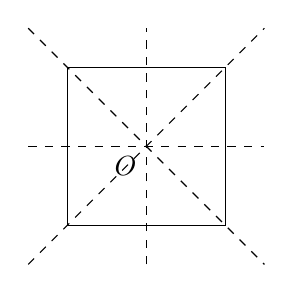
\begin{tikzpicture}
      \draw (0,0) rectangle (2,2);
      \draw[dashed] (-0.5,1)--(2.5,1);
      \draw[dashed] (1,-0.5)--(1,2.5);
      \draw[dashed] (-0.5,-0.5)--(2.5,2.5);
      \draw[dashed] (-0.5,2.5)--(2.5,-0.5);
   \draw (1,1) node [anchor=north east] {$O$};
   \end{tikzpicture}
   \caption{正方形群}
   \label{fig:group2}
\end{figure}

正方形群表示为:$\left\{ E,C_4, C_2\equiv C_4^2, C_4^3\equiv C_4^{-1},\sigma_x,\sigma_{xy},\sigma_y, \sigma_{y\overline{x}} \right\}$

\subsection{群的阶}

对称数的多少为群的阶,用符号$g$表示。对于长方形$g=4$,正文形$g=8$ , 由于$8\geq 4$ 所以正方形比长方形对称性高。


\subsection{其他例子}

\subsubsection{氢原子}

氢原子呈球对称性,如果在某一方向加上电场,则球对称性变成柱对称性。

\subsubsection{一些平面图形}


\begin{figure}[H]
   \centering
   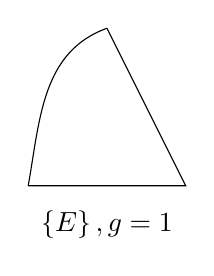
\begin{tikzpicture}
      \draw (0,0)--(2,0)--(1,2);
      \draw (0,0) to [out=80,in=200] (1,2);
      \draw (1,-0.5) node {$\left\{ E \right\}, g=1$};
   \end{tikzpicture}
   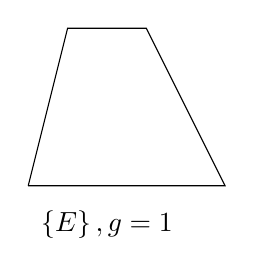
\begin{tikzpicture}
      \draw (0,0)--(2.5,0)--(1.5,2)--(0.5,2)--(0,0);
      \draw (1,-0.5) node {$\left\{ E \right\}, g=1$};
   \end{tikzpicture}
   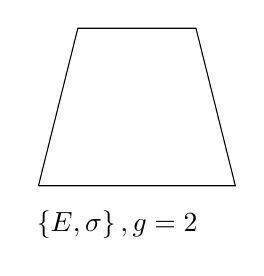
\begin{tikzpicture}
      \draw (0,0)--(2.5,0)--(2,2)--(0.5,2)--(0,0);
      \draw (1,-0.5) node {$\left\{ E , \sigma \right\}, g=2$};
   \end{tikzpicture}
   \begin{tikzpicture}
      \draw (0:1)--(120:1)--(240:1)--(360:1);
      \draw [->] (-1,0)--(1.3,0) node [anchor=north]{$x$};
      \draw [->] (0,-1)--(0,1.2) node [anchor=east]{$y$};
      \draw (120:1.2) node {$C$};
      \draw (240:1.2) node {$B$};
      \draw (0,-1.5) node {正三角形} ;
   \end{tikzpicture}
   \begin{tikzpicture}
      \draw (0:1)--(60:1)--(120:1)--(180:1)--(240:1)--(300:1)--(360:1);
      \draw (0,-1.5) node {正六边形};
   \end{tikzpicture}
   \caption{其他平面图形的群}
   \label{fig:group3}
\end{figure}

正三角形:$\left\{ E ,C_3 ,C_3^{-1},\sigma_x,\sigma_B, \sigma_C \right\}, g=6$

正六边形:课堂上老师没有具体写出,课后补充

\subsubsection{矩阵操作}

一个关于$y$轴镜面对称相当于$y'=y,x'=-x$,用矩阵可以表示为
\begin{equation}
   \sigma=\left( 
      \begin{matrix}
	 -1 & 0\\
	 0& 1
      \end{matrix}
   \right)
   \qquad
   \left( 
      \begin{matrix}
	 x'\\
	 y'
      \end{matrix}
   \right)
   =\sigma
   \left( 
      \begin{matrix}
	 x\\
	 y
      \end{matrix}
   \right)
   =\left( 
      \begin{matrix}
	 -1 & 0\\
	 0& 1
      \end{matrix}
   \right)
   \left( 
      \begin{matrix}
	 x\\
	 y
      \end{matrix}
   \right)
   \label{eq:jmdc1}
\end{equation}

\subsubsection{周期性}

固体物理中没有正五边形晶体,周期性与对称性相互联系与制约。但是1984年发现5度对称性的准晶,而准晶不是晶体。晶体周期性结构称为晶胞,一个cell.

\subsubsection{微信群和数学上的群}

微信群: 对元素而言为集合,可以多也可以少,集合(set) 

数学上的群: 满足所有对称性条件的集合。

\subsection{群的定义}

\begin{definition}{群}
   数学对象(群元)的集合$\left\{ A,B,C,\cdots \right\}$,其中有一个与次序有关的运算(群乘)$AB=C$ ,若满足下列四个条件,该集合称为群(group , 记作G)
   \begin{enumerate}
      \item 封闭性
      \item 结合律成立:$A(BC)=(AB)C$
      \item 单位元存在:$EA=AE=A$
      \item 逆元存在:$A^{-1}A=AA^{-1}=E$
   \end{enumerate}
   \label{def:group1}
\end{definition}

\begin{note}
   若群乘满足交换律,称作交换群或阿贝尔群
\end{note}

\subsection{连续操作}

以正三角形为例:一般操作都是在$2\pi$角内的。

\begin{figure}[H]
   \centering
   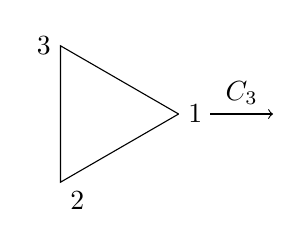
\begin{tikzpicture}
      \draw (0:1)--(120:1)--(240:1)--(360:1);
      \draw (0:1) node [anchor=west]{$1$};
      \draw (120:1) node [anchor=east]{$3$};
      \draw (240:1) node [anchor=north west]{$2$};
      \draw [->](0:1.4)--(0:2.2);
      \draw (0:1.8) node [anchor=south] {$C_3$};
   \end{tikzpicture}
   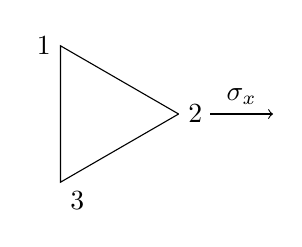
\begin{tikzpicture}
      \draw (0:1)--(120:1)--(240:1)--(360:1);
      \draw (0:1) node [anchor=west]{$2$};
      \draw (120:1) node [anchor=east]{$1$};
      \draw (240:1) node [anchor=north west]{$3$};
      \draw [->](0:1.4)--(0:2.2);
      \draw (0:1.8) node [anchor=south] {$\sigma_x$};
   \end{tikzpicture}
   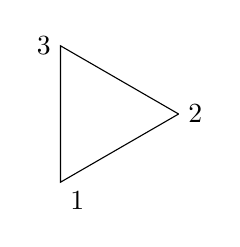
\begin{tikzpicture}
      \draw (0:1)--(120:1)--(240:1)--(360:1);
      \draw (0:1) node [anchor=west]{$2$};
      \draw (120:1) node [anchor=east]{$3$};
      \draw (240:1) node [anchor=north west]{$1$};
   \end{tikzpicture}
   \caption{连续操作 $\sigma_x C_3$}
   \label{fig:lxcz0}
\end{figure}

\begin{note}
由以上变换可得:$\sigma_x C_3=\sigma_C$
\end{note}

\begin{figure}[H]
   \centering
   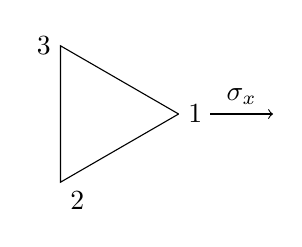
\begin{tikzpicture}
      \draw (0:1)--(120:1)--(240:1)--(360:1);
      \draw (0:1) node [anchor=west]{$1$};
      \draw (120:1) node [anchor=east]{$3$};
      \draw (240:1) node [anchor=north west]{$2$};
      \draw [->](0:1.4)--(0:2.2);
      \draw (0:1.8) node [anchor=south] {$\sigma_x$};
   \end{tikzpicture}
   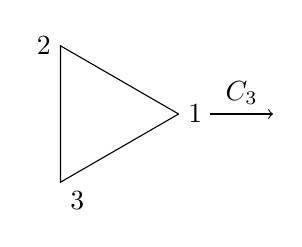
\begin{tikzpicture}
      \draw (0:1)--(120:1)--(240:1)--(360:1);
      \draw (0:1) node [anchor=west]{$1$};
      \draw (120:1) node [anchor=east]{$2$};
      \draw (240:1) node [anchor=north west]{$3$};
      \draw [->](0:1.4)--(0:2.2);
      \draw (0:1.8) node [anchor=south] {$C_3$};
   \end{tikzpicture}
   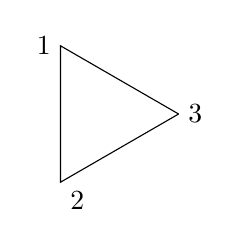
\begin{tikzpicture}
      \draw (0:1)--(120:1)--(240:1)--(360:1);
      \draw (0:1) node [anchor=west]{$3$};
      \draw (120:1) node [anchor=east]{$1$};
      \draw (240:1) node [anchor=north west]{$2$};
   \end{tikzpicture}
   \caption{连续操作 $\sigma_x C_3$}
   \label{fig:lxcz1}
\end{figure}

\begin{note}
由以上变换可得:$C_3\sigma_x =\sigma_B$
\end{note}

\subsection{群的分类}

\subsubsection{群分类}

\begin{enumerate}
   \item 根据群阶$g$划分:
      \begin{enumerate}
	 \item 有限群
	 \item 无限群(离散的无限群和连续群)
      \end{enumerate}
   \item 物理学中的群论课:
      \begin{enumerate}
	 \item 固体群
	 \item 李群
      \end{enumerate}
   \item 若干具体的群举例:
      \begin{enumerate}
	 \item 群元特征:
	    \begin{enumerate}
	       \item 普通的群
	       \item 方阵群
	       \item 对称操作群
	       \item 置换群等
	    \end{enumerate}
      \end{enumerate}
   \item 循环群:群元自乘若干次
   \item 阿贝尔群:可交换群
\end{enumerate}

\subsubsection{一些例子}

\begin{enumerate}
   \item 整数群:若群乘为加法,则构成群
   \item 整数群:若群乘为乘法,则不是群
   \item 正有理数:若群乘为乘法,则构成群
   \item $\left\{ -1,1 \right\}$ 群乘为乘法,构成群
   \item $\left\{ 1,i,i^2=-1,i^3=-i \right\}$ 群乘为乘法,构成四阶群
\end{enumerate}

\subsection{作业}
\begin{exercise}
   列出正三角形全部对称操作(正三角形群),并做出至少5个连续操作(群乘)。
\end{exercise}
\begin{exercise}
   列出正方形的全部对称操作(正方形群),并做出至少5个连续操作(群乘)。
\end{exercise}
\begin{exercise}
   说明正三角形群不是阿贝尔群
\end{exercise}

\end{document}


